\documentclass[a4paper,12pt]{article}
\usepackage[a4paper,top=1.3cm,bottom=2cm,left=1.5cm,right=1.5cm,marginparwidth=0.75cm]{geometry}

% Пакеты
\usepackage{mathtext} 
\usepackage{setspace}
\usepackage{tabularx}
\usepackage{cmap}
\usepackage{longtable}
\usepackage{icomma}
\usepackage{euscript}
\usepackage{float}
\usepackage{cutwin}
\usepackage{mathrsfs}
\usepackage{adjustbox}
\usepackage{dashbox}
\usepackage[normalem]{ulem}
\usepackage[T2A]{fontenc}			
\usepackage[utf8]{inputenc}                 %!  закрепляет кодировку utf8
\usepackage[english,russian]{babel}         %!  подключает русский и английский
%математические шрифты:
\usepackage{amsmath,amsfonts,amssymb,amsthm,mathrsfs,mathtools} 
\usepackage[colorlinks, linkcolor = purple]{hyperref}      %!  оглавление для панели навигации по PDF-документу + гиперссылки
\usepackage{xcolor}                         %!  добавляет цвета
\usepackage{enumitem}                       %!  задание макета перечня.
\usepackage{xpatch}                         %?  работа с renewcommand и макросами              
\usepackage{cancel}                         %   зачёкивания текста (!!!) для slash-нотации использовать \usepackage{slashed}!!
\usepackage{upgreek}                        %   заглавные греческие буквы
\usepackage{lipsum}                         %?  для вставки кучи текста при форматировании
\usepackage[version=4]{mhchem}              %   химические формулы
\usepackage{multirow}                       %   объединение строк в матрицах
\usepackage{stackengine}                    %   stack символов
\usepackage{tikz}                           %!  рисунки
\usetikzlibrary{positioning}                %?  библиотека для тикза 
\usepackage{titletoc}                       %!  форматирование содержания и заголовков
\usepackage{titlesec}                       %!  форматирование содержания и заголовков
\usepackage{wrapfig}                        %   обтекание таблиц и рисунков
\usepackage{chngcntr}                       %!  для setcounter
\usepackage{fancyhdr}                       %!  для колонтитулов
\usepackage{makecell}                       %?  матрицы с разными выравниваниями и т.п
\usepackage{indentfirst}                    %   добавить indent перед первым 
\usepackage{tocloft}                        %?  изменение названий глав и разделов                       
\usepackage{soul}                           %   типографические примочки, типо зачёркивания и подчёркивания
\usepackage[stable]{footmisc}               %?  продвинутые сноски
\usepackage{subfig}                         %   несколько картинок рядом
%  задаёт поля страниц

% pgf plots
% \usepackage{pgfplots}
% \pgfplotsset{compat=1.17}

\mathtoolsset{showonlyrefs=true}

%Обозначения теорем и т.п
\theoremstyle{definition}
\newtheorem*{definition}{Определение}
\newtheorem{statement}{Предложение}[section]
\newtheorem{lemma}{Лемма}[section]
\newtheorem{theorem}{Теорема}[section]
\newtheorem*{theoremn}{Теорема}
\newtheorem*{corollary}{Следствие}
\newtheorem*{example}{Пример}
\newtheorem*{note}{Замечание}
\newtheorem*{problem}{Задача}

%Шарабара для содержания и внешнего вида нумерации
\counterwithout{footnote}{section}\DeclareRobustCommand{\divby}{%
	\mathrel{\text{\vbox{\baselineskip.65ex\lineskiplimit0pt\hbox{.}\hbox{.}\hbox{.}}}}%
}



%Толерантный квадратик чтд
%\makeatletter \renewenvironment{proof}[1][\proofname]{\par\pushQED{\qed}\normalfont\topsep6\p@\@plus6\p@\relax\trivlist\item[\hskip\labelsep\bfseries#1\@addpunct{.}]\ignorespaces}{\popQED\endtrivlist\@endpefalse} \makeatother
%\renewcommand\qedsymbol{$\squareulblack$}
%\newcommand{\usubseteq}{\mathbin{\rotatebox[origin=c]{90}{$\subset$}}}
%\DeclareFontEncoding{LS2}{}{\noaccents@}
%\DeclareFontSubstitution{LS2}{stix}{m}{n}
%\DeclareSymbolFont{arrows3}{LS2}{stixtt}{m}{n}
%\DeclareMathSymbol{\squareulblack}{\mathord}{arrows3}{"88}

%Разные операторы и символы
\newcommand{\dotpr}[2]{\bra{#1}\ket{#2}}
\let\AA\relax
%\let\oldvarphi\phi %оно делает так, что \phi становится правильным фи
%\let\phi\varphi
%\let\varphi\oldvarphi
\let\emptyset\varnothing
\DeclareMathOperator*{\esssup}{ess sup}
\DeclareMathOperator*{\ord}{ord}
\DeclareMathOperator*{\supp}{supp}
\DeclareMathOperator*{\pr}{pr}
\DeclareMathOperator*{\Ker}{Ker}
\DeclareMathOperator*{\Vol}{Vol}
\DeclareMathOperator*{\rg}{rk}
\DeclareMathOperator*{\Ima}{Im}
\DeclareMathOperator*{\Alt}{Alt}
\DeclareMathOperator*{\Sym}{Sym}
\newcommand{\eqdef}{\stackrel{\text{\tiny{def}}}{=}}
\newcommand{\pp}{\partial}
\newcommand{\AA}{\mathcal{A}}
\newcommand{\BB}{\mathcal{B}}
\newcommand{\MM}{\mathbb{M}}
\newcommand{\NN}{\mathbb{N}}
\newcommand{\ZZ}{\mathbb{Z}}
\newcommand{\QQ}{\mathbb{Q}}
\newcommand{\RR}{\mathbb{R}}
\newcommand{\CC}{\mathbb{C}}
\newcommand{\FFF}{\mathbb{F}}
\newcommand{\DD}{\mathcal{D}}
\newcommand{\FF}{\mathcal{F}}
\newcommand{\sS}{\mathcal{S}}
\newcommand*\circled[1]{\tikz[baseline=(char.base)]{
		\node[shape=circle,draw,inner sep=2pt] (char) {#1};}}

\graphicspath{ {./images/2.2.2} }


\title{Измерение теплопроводности воздуха при разных давлениях (2.2.2)}
\author{Павлушкин Вячеслав}
\date{\today}


\begin{document}
	\maketitle
	
	\section{Аннотация}
	В данной работе мы наблюдаем за изменением теплопроводности воздуха с помощью платиновой нити. Определяем коэффициент теплопередачи при высоких и низких давлениях
	
	\section{Теоретические сведения}
	
	Теплопроводность — это процесс передачи энергии от нагретых частей системы к холодным за счет хаотического движения частиц среды (молекул, атомов и т.п.). В газах теплопроводность осуществляется за счет непосредственной передачи кинетической энергии от быстрых молекул к медленным при их столкновениях. Перенос тепла описывается законом Фурье:
	\begin{equation}
		\vec{q} = -\varkappa\cdot\nabla T,
	\end{equation}
	где $\vec{q}$ --- плотность потока энергии, $\varkappa$ --- коэффициент теплопроводности. Система, используемая в данной установке, имеет цилиндрическую симметрию (пренебрегая краевым эффектами), поэтому имеем 
	\begin{equation}
		q = -\varkappa\frac{dT}{dr},
	\end{equation}
	где $r$ --- расстояние от оси симметрии системы.
	
	Закон Фурье применим при условиях $$\lambda\ll r\quad \text{и}\quad \lambda |\nabla T|\ll T, $$
	где $\lambda$--- длина свободного пробега молекул газа, а $r$--- характерный размер системы.
	
	Для количественного описания способности некоторой системы к теплопередаче в целом используют коэффициент $K$, называемый \emph{тепловым сопротивлением}, равный отношению перепада температур $\Delta T$ в системе к полному потоку энергии $Q$ [Вт] через нее:
	\begin{equation}
		K = \frac{\Delta T}{Q}
	\end{equation}
	
	
	\section{Экспериментальная установка}
	\begin{wrapfigure}{L}{8cm}
		\centering
		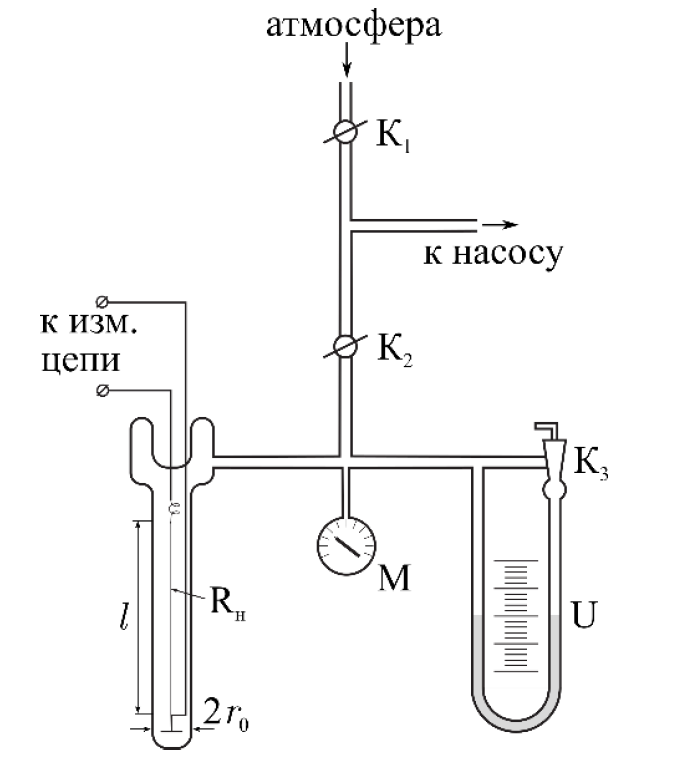
\includegraphics[scale = 0.6]{ustan}
		\caption{Вакуумная часть установки}
		\label{facility}
	\end{wrapfigure}
	Схема установки приведена на рис. \eqref{facility} Внутренняя полость тонкостенной цилиндрической стеклянной колбы, на оси которой натянута металлическая (платиновая) нить, подсоединена к вакуумной установке. Колба заполнена воздухом и расположена вертикально. Контактные провода от нити выведены наружу через стеклянную вакуумную «слезку».
	
	Вакуумная установка состоит из форвакуумного насоса, стрелочного вакуумметра $M$ и U-образного масляного манометра. Вакуумметр служит для измерения высоких давлений вплоть до ~10 торр (он показывает разность давлений между установкой и атмосферой, так что нуль на его шкале соответствует атмосферному давлению в установке). U-образный манометр заполнен маслом с плотностью 0,885 г/см$^3$ и предназначен для измерения низких давлений (вплоть до ~0,1 торр). Кран К$_1$ служит для соединения установки и насоса с атмосферой, кран К$_2$ — для отсоединения откачиваемого объема от насоса, кран К$_3$ — для соединения колен U-образного манометра.
	
	Металлическая нить служит как источником тепла, так и датчиком температуры (термометром сопротивления). В рабочем диапазоне температур (20–40 $^\circ C$) сопротивление платины зависит от температуры практически линейно:
	\begin{equation}
		R(t)=R_{0}\left(1+\alpha_{0} t\right)
	\end{equation}
	где $t$ --- температура в $^\circ C$, $R_0$--- сопротивление про 0$^\circ C$, и
	\begin{equation}
		\alpha_{0}=\frac{1}{R_{0}} \frac{d R}{d t}=3,92 \cdot 10^{-3} ~^\circ C^{-1}.
	\end{equation}
	
	\begin{figure}[!h]
		\centering
		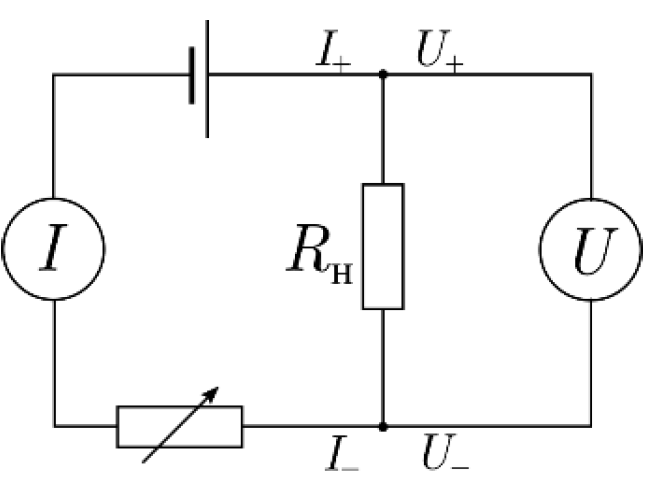
\includegraphics[width=50mm]{elustan}
		\caption{Электрическая схема измерений}
		\label{elfacility}
	\end{figure}
	
	Электрическая схема установки приведена на рис. \eqref{elfacility} Ток $I$ через сопротивление $R_\text{н}$ и напряжение $U$ на нем измеряются цифровыми мультиметрами, один из которых работает в режиме амперметра, а другой — вольтметра. Сопротивление $R_\text{н}$ находится по закону Ома. Те же измерения позволяют определить мощность нагрева проволоки как джоулево тепло. Ток в цепи регулируется с помощью магазина сопротивлений, включенного последовательно с источником тока.
	\section{Ход работы}
	\begin{enumerate}
		\item Оценим, когда длина свободного пробега сравняется с радиусом нити:
		\begin{equation*}
			P_1 \approx \frac{kT}{r_{н} \pi d^2}\approx 430\text{ Па}.
		\end{equation*}
	\item Проведя подготовку экспериментальной установки измерим измерим зависимость сопротивления нити от подаваемой на нее мощности:
	\begin{table}[H]
		\begin{center}
			\begin{tabular}{|c|c|c|c|}
				\hline
				$I,$ мА & $U,$ В& $R,$ Ом & $Q,\: 10^{-6}$ Вт \\ \hline
				10.03 & 0.118 & 11.76 & 1.18 \\ \hline
				20.16 & 0.237 & 11.76 & 4.78 \\ \hline
				30.06 & 0.354 & 11.78 & 10.64 \\ \hline
				40.07 & 0.474 & 11.83 & 18.99 \\ \hline
				50.04 & 0.596 & 11.91 & 29.82 \\ \hline
				60.06 & 0.72 & 11.99 & 43.24 \\ \hline
				70.0 & 0.846 & 12.09 & 59.22 \\ \hline
			\end{tabular}
		\end{center}
	\end{table}
	\begin{figure}[!h]
		\centering
		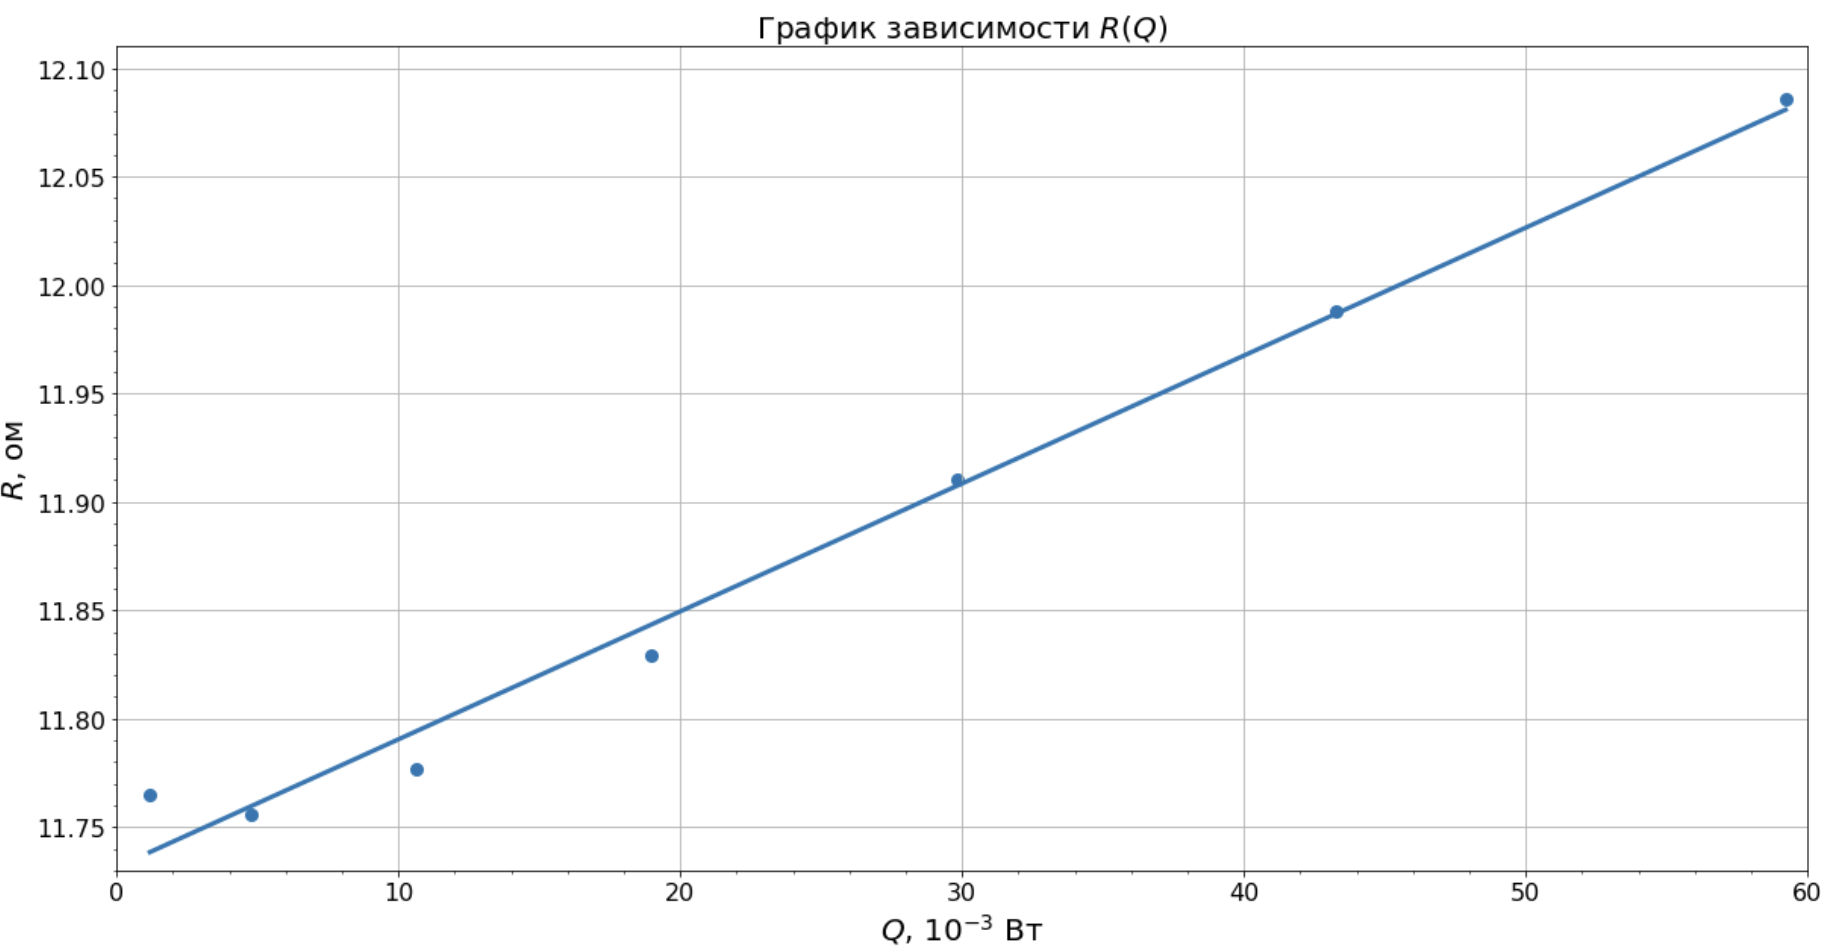
\includegraphics[scale = 0.55]{rq}
		\caption{График зависимости $R(Q)$}
		\label{graph1}
	\end{figure}
	\item Экстраполируя график \eqref{graph1} к нулевому значению, получаем:
	\begin{align*}
		R_{к} = (11,73 \pm 0,009)\text{ Ом,} && R_0 = (10,63\pm0,008)\text{ Ом,} && R_{max} = (12,98\pm0,010)\text{ Ом.}
	\end{align*}
	\item Проводим измерения, аналогичные пункту 2, только теперь  еще определяем температуру:
	\begin{table}[H]
		\centering
		\begin{minipage}{.49\linewidth}
			\centering
			\begin{tabular}{|c|c|c|c|}
				\hline
				\multicolumn{4}{|c|}{$P_1 = 69$ Па}\\
				\hline
				$I,$ мА & $U,$ В& $T,$ $^\circ$С & $Q,\: 10^{-6}$ Вт \\ \hline
				10 & 0.117 & 25.68 & 1.17 \\ \hline
				20 & 0.235 & 26.88 & 4.7 \\ \hline
				30 & 0.356 & 29.68 & 10.68 \\ \hline
				40 & 0.48 & 32.88 & 19.2 \\ \hline
				50 & 0.609 & 37.2 & 30.45 \\ \hline
				60 & 0.744 & 42.48 & 44.64 \\ \hline
				70 & 0.887 & 48.99 & 62.09 \\ \hline
			\end{tabular}
		\end{minipage}
		\begin{minipage}{.49\linewidth}
			\centering
			\begin{tabular}{|c|c|c|c|}
				\hline
				\multicolumn{4}{|c|}{$P_2 = 86$ Па}\\
				\hline
				$I,$ мА & $U,$ В& $T,$ $^\circ$С & $Q,\: 10^{-6}$ Вт \\ \hline
				10 & 0.118 & 28.08 & 1.18 \\ \hline
				20 & 0.235 & 26.88 & 4.7 \\ \hline
				30 & 0.356 & 29.68 & 10.68 \\ \hline
				40 & 0.478 & 31.68 & 19.12 \\ \hline
				50 & 0.606 & 35.76 & 30.3 \\ \hline
				60 & 0.739 & 40.48 & 44.34 \\ \hline
				70 & 0.879 & 46.25 & 61.53 \\ \hline
			\end{tabular}
		\end{minipage}
		
		\caption{Результаты измерений для низких давлений}
		\label{lowp}
	\end{table}
	Остальные таблицы для низких давлений можно найти в приложении.
	
	График зависимости $T_{н}(Q)$, для низких давлений:
	\begin{figure}[!h]
		\centering
		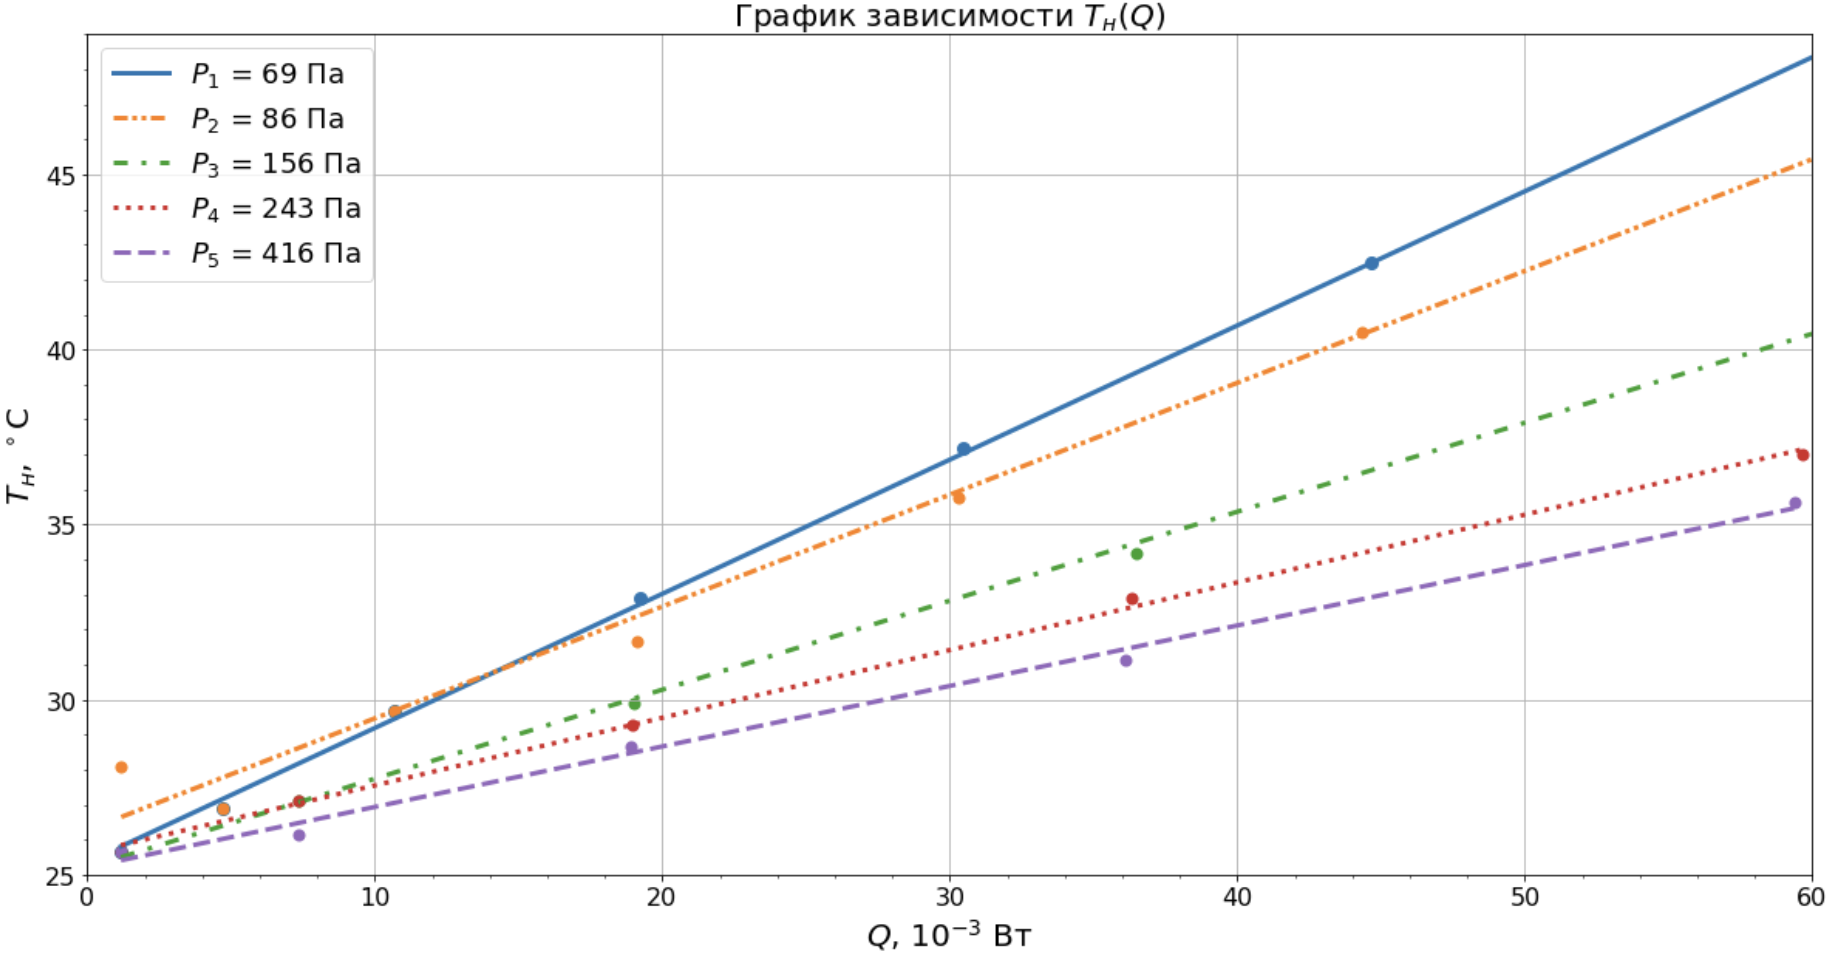
\includegraphics[scale = 0.55]{tq1}
		%\caption{График зависимости $T_{н}(Q)$}
		\label{graph2}
	\end{figure}
	
	Полученные для этих давлений коэффициенты теплового сопротивления:
	\bgroup
	\def\arraystretch{1.2}%
	\begin{table}[H]
		\centering
		\begin{tabular}{|c|c|c|c|c|c|}
			\hline
			~ &1&2&3&4&5\\\hline
			$P,$ Па&69&86&156&243&416\\ \hline
			$K,\: 10^3$ $\frac{^\circ\text{С}}{\text{Вт}}$& 383.1&319.4&254.1&193.3&172.7\\\hline
			$\sigma_K,\: 10^3$ $\frac{^\circ\text{С}}{\text{Вт}}$ & 0.4& 0.3& 0.3& 0.2&0.2\\\hline
		\end{tabular}
		\caption{Коэффициенты теплового сопротивления для низких давлений}
		\label{tablow}
	\end{table}
	\egroup
	То же самое для высоких давлений:
	\begin{table}[H]
		\centering
		\begin{minipage}{.49\linewidth}
			\centering
			\begin{tabular}{|c|c|c|c|}
				\hline
				\multicolumn{4}{|c|}{$P_1 = 1335$ Па}\\
				\hline
				$I,$ мА & $U,$ В& $T,$ $^\circ$С & $Q,\: 10^{-6}$ Вт \\ \hline
				10 & 0.117 & 25.68 & 1.17 \\ \hline
				25 & 0.293 & 26.16 & 7.32 \\ \hline
				40 & 0.471 & 27.48 & 18.84 \\ \hline
				55 & 0.654 & 30.26 & 35.97 \\ \hline
				70 & 0.842 & 33.56 & 58.94 \\ \hline
			\end{tabular}
		\end{minipage}
		\begin{minipage}{.49\linewidth}
			\centering
			\begin{tabular}{|c|c|c|c|}
				\hline
				\multicolumn{4}{|c|}{$P_2 = 11025$ Па}\\
				\hline
				$I,$ мА & $U,$ В& $T,$ $^\circ$С & $Q,\: 10^{-6}$ Вт \\ \hline
				10 & 0.117 & 25.68 & 1.17 \\ \hline
				25 & 0.293 & 26.16 & 7.32 \\ \hline
				40 & 0.471 & 27.48 & 18.84 \\ \hline
				55 & 0.654 & 30.26 & 35.97 \\ \hline
				70 & 0.841 & 33.22 & 58.87 \\ \hline
			\end{tabular}
		\end{minipage}
		
		\caption{Результаты измерений для высоких давлений}
		\label{highp}
	\end{table}
	\begin{figure}[H]
		\centering
		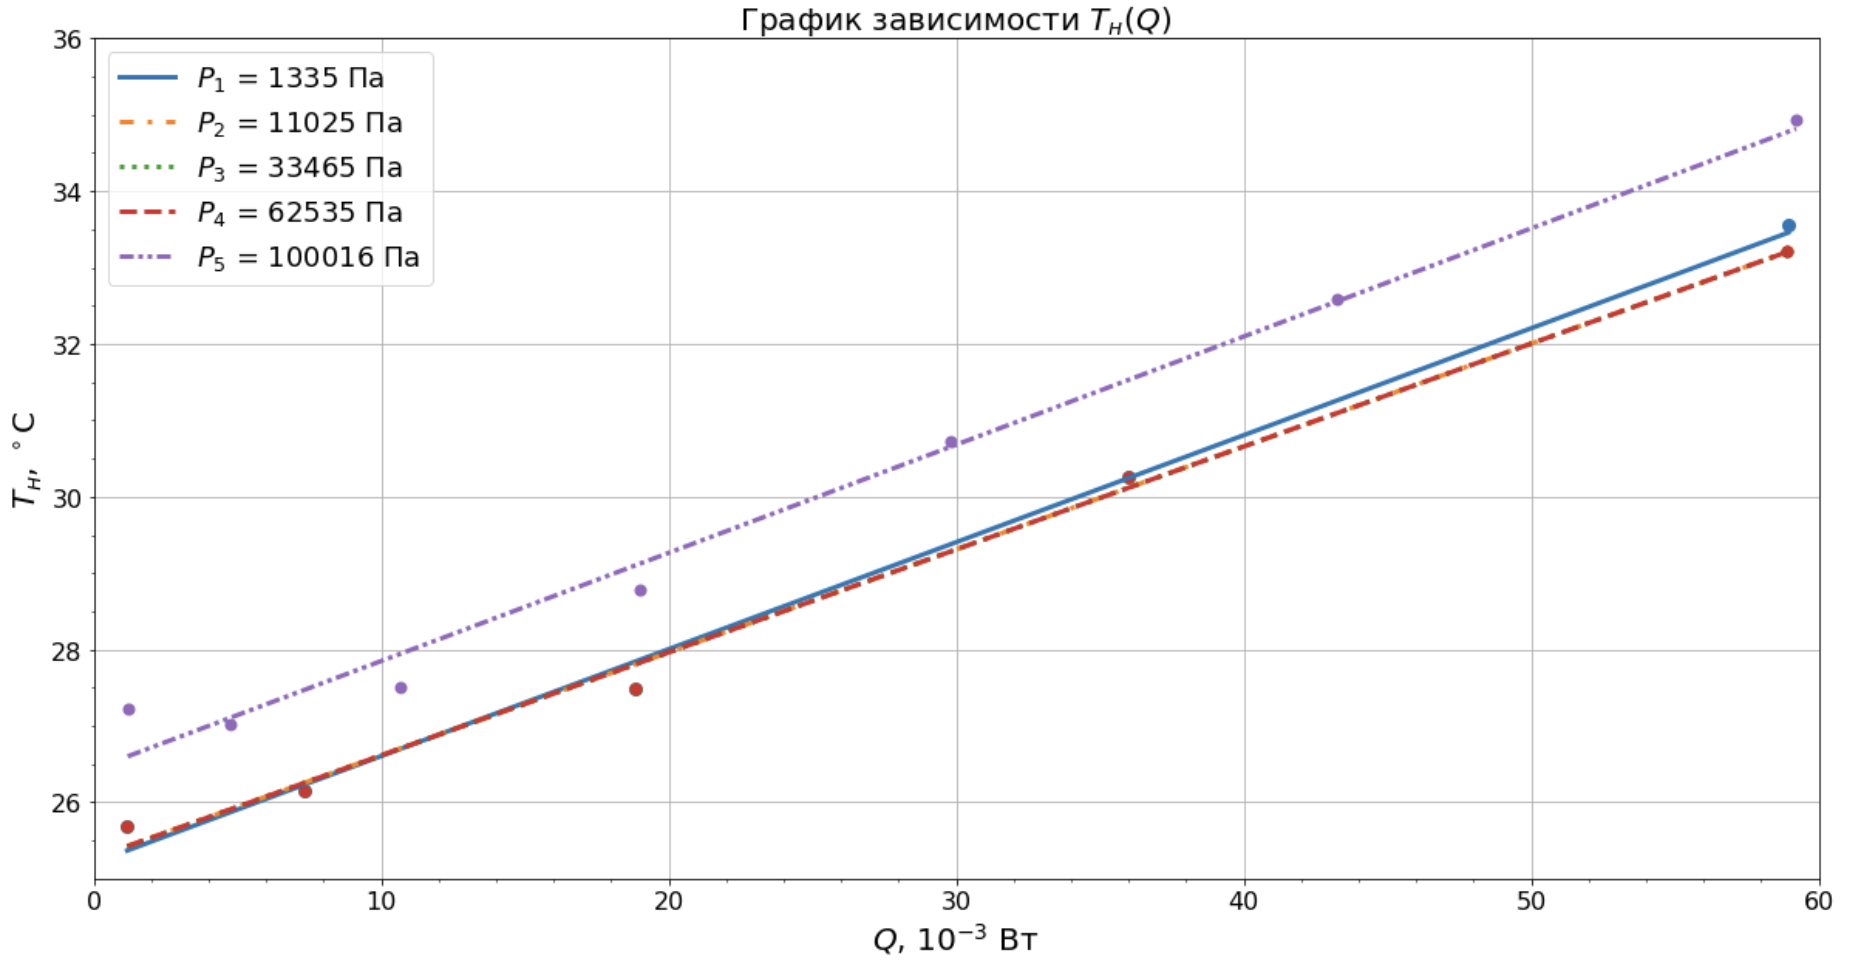
\includegraphics[scale = 0.55]{tq2}
		%\caption{График зависимости $T_{н}(Q)$}
		\label{graph3}
	\end{figure}
	Коэффициенты теплового сопротивления полученные для высоких давлений :
	\bgroup
	\def\arraystretch{1.2}%
	\begin{table}[H]
		\centering
		\begin{tabular}{|c|c|c|c|c|c|}
			\hline
			~ &1&2&3&4&5\\\hline
			$P,$ Па&1335&11025&33465&62535&100016\\ \hline
			$K,$ $\frac{^\circ\text{С}}{\text{Вт}}$& 140.0&134.7&134.7&134.7&141.6\\\hline
			$\sigma_K,$ $\frac{^\circ\text{С}}{\text{Вт}}$ & 0.2& 0.1& 0.1& 0.1&0.2\\\hline
		\end{tabular}
		\caption{Коэффициенты теплового сопротивления для высоких давлений}
		\label{tabhigh}
	\end{table}
	\egroup
	\item По полученным данным построим график зависимости теплового сопротивления системы от давления $K(P):$
	
	\begin{table}[H]
		\centering
		\begin{minipage}{.49\linewidth}
			\centering
			\begin{figure}[H]
				\centering
				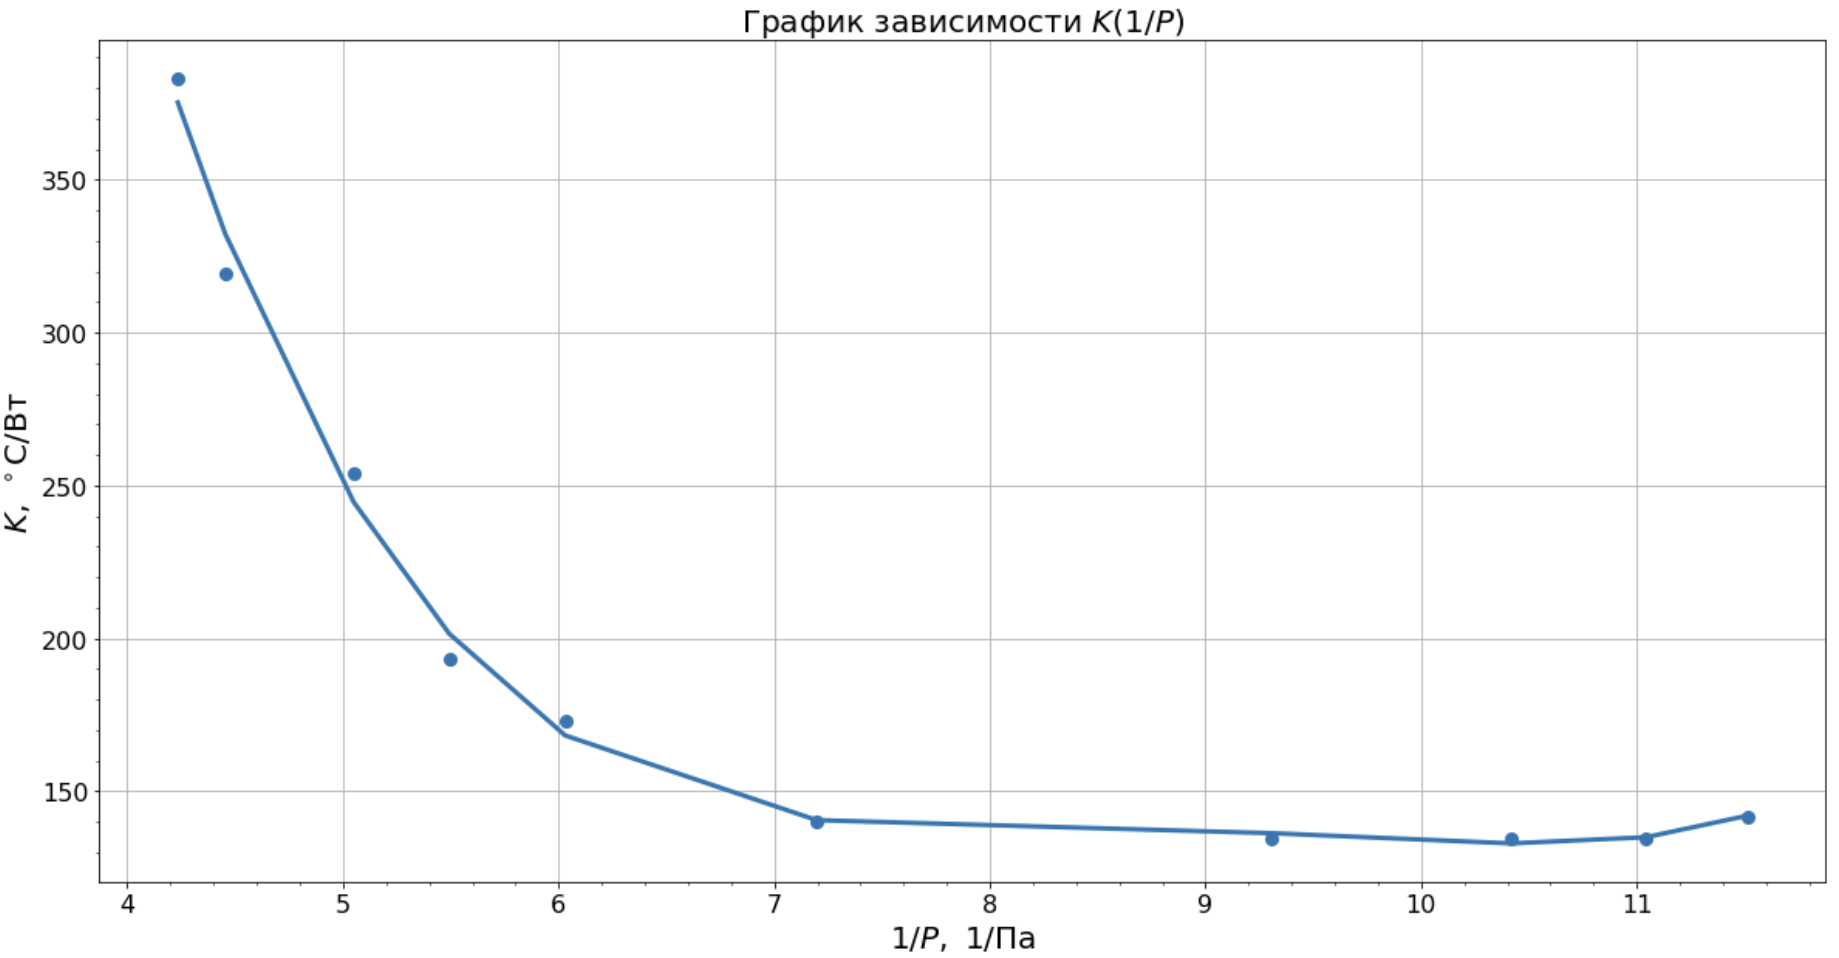
\includegraphics[scale = 0.25]{kp}
				%\caption{График зависимости $T_{н}(Q)$}
				%\label{graph4}
			\end{figure}
		\end{minipage}
		\begin{minipage}{.49\linewidth}
			\centering
			\begin{figure}[H]
				\centering
				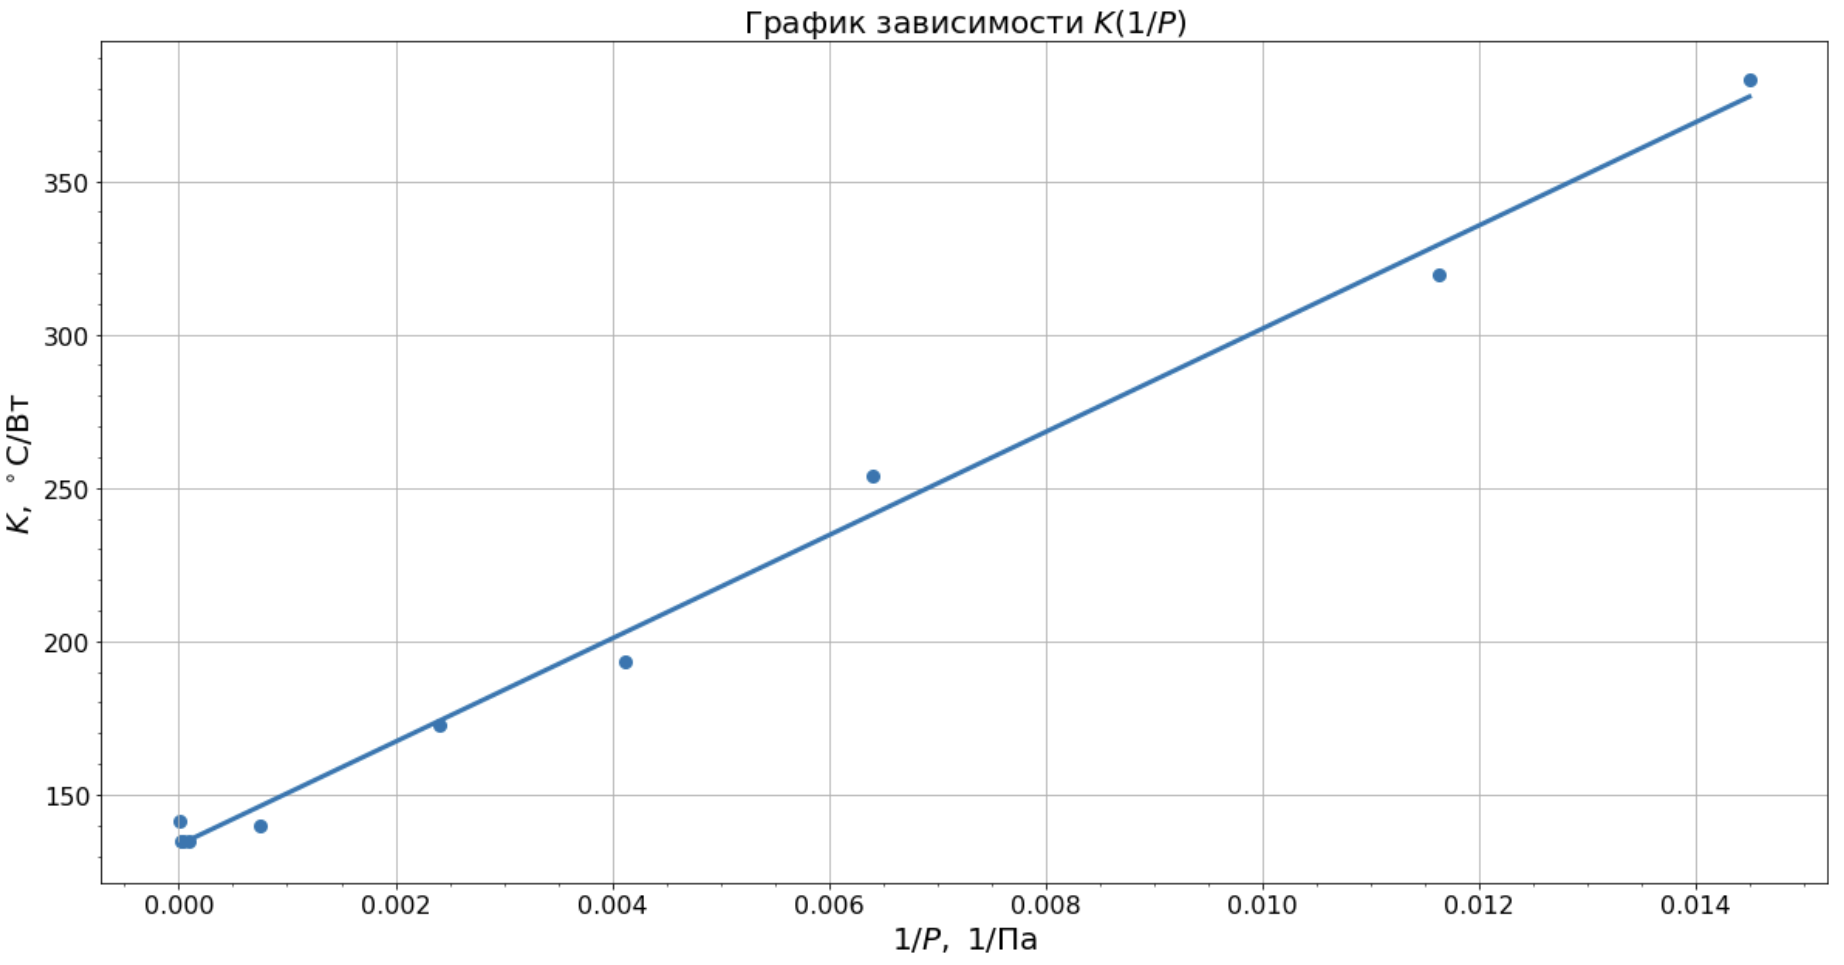
\includegraphics[scale = 0.25]{kp2}
				%\caption{График зависимости $T_{н}(Q)$}
				%\label{graph5}
			\end{figure}
		\end{minipage}
	\end{table}
	

	И, действительно, заметна область, где теплопередача перестает зависеть от давления $(K = const)$.

	По графику можно найти $K_\infty = (134 \pm 1)$ $\text{К}/\text{Вт}$, и по графику зависимости $K(1/P)$, можно найти $A = (16800\pm 600)$ $\text{К} / \text{Вт}\cdot\text{Па}$. Теперь, с помощью полученного $K_\infty$, найдем коэффициент теплопроводности воздуха:
	\begin{equation*}
		\varkappa \approx \frac{1}{2\pi LK_\infty} \ln\frac{R}{r_{\text{н}}} =  (28.6\pm0.2)\cdot 10^{-3}\: \text{Вт}/\text{м}\cdot\text{К}.
	\end{equation*}

	\item Так же, с помощью $A$, можно получить коэффициент аккомодации:
	\begin{equation*}
		s =\frac{1}{Lr_\text{н} C_V \cdot A} \sqrt {\frac{\mu RT_\text{к}}{2\pi}} \approx 0,65 \pm 0,06 
	\end{equation*}
	\end{enumerate}
	\section{Вывод}
	
	В работе был проверен метод по определению коэффициента теплопроводности воздуха при комнатной температуре в зависимости от давления.
	
	Был получен коэффициент теплопроводности:
	\begin{equation*}
		\varkappa  =  (28.6\pm0.2)\cdot 10^{-3}\: \text{Вт}/\text{м}\cdot\text{К}.
	\end{equation*}

	Тепловое сопротивление:
	\begin{equation*}
		K_\infty = (134 \pm 1)\:\text{К}/\text{Вт}
	\end{equation*}

	И коэффициент аккомодации:
	\begin{equation*}
		s = 0,65 \pm 0,06
	\end{equation*}
	
	Также проверена теория о том, что при высоком давлении теплопередача перестает от него зависеть.
	
\end{document}